\documentclass[12pt, titlepage, twoside, a4paper]{report}
\usepackage{geometry}
\usepackage{fancyhdr}
\usepackage{graphicx}
\usepackage{textcomp}
\usepackage{float}
\usepackage{amssymb}
\usepackage{sidecap}
\usepackage[notes]{biblatex-chicago}
\bibliography{./references/references}
\usepackage{amsmath}
\usepackage[nottoc]{tocbibind}
\graphicspath{ {images/} }
\pagestyle{fancy}
\fancyhead{}
\fancyhead[LO,RE]{Liars, Truth-tellers, and Interactive Identification}
\fancyhead[RO,LE]{Perry, Axford, Cairns}
\fancyfoot{}
\fancyfoot[LE,RO]{\thepage}
\fancyfoot[LO,CE]{Section \thesection}

\title{
{What Kinds of Liars and Truth-tellers Exist, and How Can They Be Identified Through Interaction?} \newline \newline
{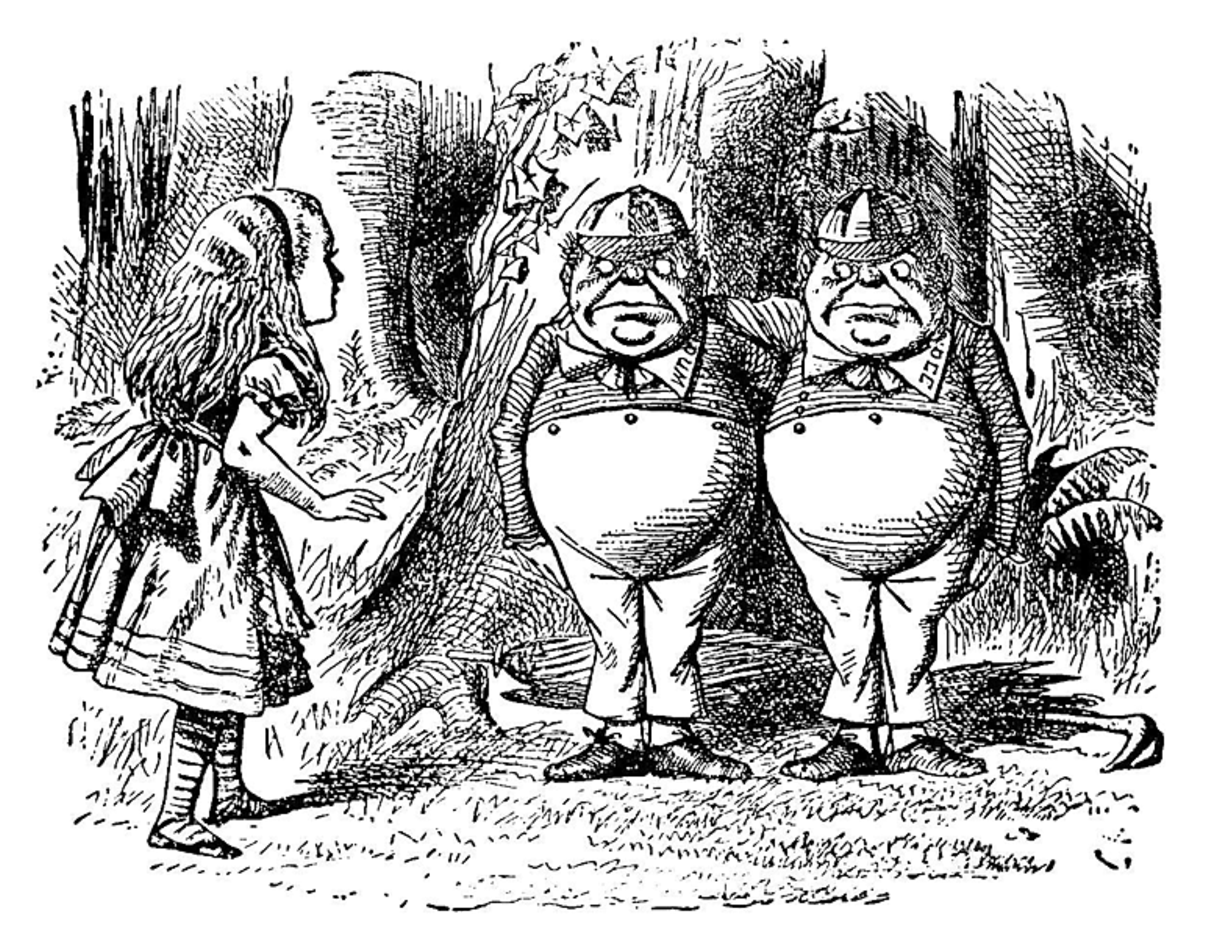
\includegraphics[width=11cm]{alice.eps}}\\
{\large University of Auckland}\\
{\large Philosophy 315}\\
\author{Emma Perry, Forrest Axford, Jason Cairns}}

\newcommand{\true}{$T\text{\textmusicalnote}$}
\newcommand{\false}{$F\text{\textmusicalnote}$}

\begin{document}

\maketitle
\tableofcontents
\newpage
\section*{Abstract}
Truth-telling and lying come in many different forms - we intend to develop a taxonomy through the exploration of some intuitive and counter-intuitive types, and determine how an agent's category can be identified through interaction.

\section*{A Note on Belief}
It’s worth noting that the way in which one determines belief can  have drastic impacts on logical systems of liars and truth tellers which consider belief.\autocite{sep-logic-action} If a Lockean conception of belief is used, $\tau$ being set to anything less than 0.5 can result in the speaker being both a liar and truth-teller simultaneously if using a system in which liars are those who say something they believe not to be true and truth-tellers are those that say something they believe to be true.\autocite{sep-logic-epistemic} 

\chapter{Basic Types}
\begin{table}[h]
\begin{tabular}{lp{9cm}l}
\hline
   & Description                                                                        & Logical formulation                               \\ \hline
1  & Truth-telling as saying something which is true in reality                         & (\true$\psi \to \psi$)                            \\
2  & Lying as saying something which is not the case in reality                         & (\false$\psi \to \neg \psi$)                      \\ \hline
3  & Truth-telling as saying something sincerely                                        & (\true$\psi \to B_T \psi$)                     \\
4  & Lying as saying something insincerely                                              & (\false$\psi \to \neg B_L \psi$)               \\
5  & Lying as saying something believed to be untrue                                    & (\false$\psi \to  B_L \neg \psi$)              \\ \hline
6  & Truth-telling as saying something that is both true in reality and sincere         & (\true$\psi \to (\psi \wedge B_T \psi)$)       \\
7  & Lying as saying something that is both untrue in reality and insincere             & (\false$\psi \to (\psi \wedge \neg B_L \psi)$) \\
8  & Lying as saying something that is both untrue in reality and believed to be untrue & (\false$\psi \to (\psi \vee B_L \neg \psi)$)   \\ \hline
9  & Truth-telling as imparting knowledge                                               & (\true$\psi \to K_T \psi$)                     \\
10 & Lying as imparting what one knows to be false                                      & (\false$\psi \to K_L \neg \psi$)               \\ \hline
\end{tabular}
\end{table}

\section{Identifying Liars and Truth-tellers through an Update Game}
A simple method of discernment between liars and truth-tellers is through the scope of an update game. For each of these games the agents must adhere to four key conditions:
\begin{itemize}
\item An agent must make a statement to begin the game
\item Statements must be made from one agent to at least one other
\item The second agent $x$ is taken as a reliable source by the first agent $a$:\\
$(x\text{\textmusicalnote}_a \psi \to (\psi \wedge K_a \psi))$
\item An agent must make a statement if possible whenever asked (statements can change, but means of truth-telling cannot change)
\end{itemize}

\subsection{Interaction with Alan Truering and Ada Love-Lies}
Let an omniscient truth-teller be an agent named Alan Truering, and an omniscient liar be named Ada Love-Lies\\
If you know an agent is Ada Love-Lies or Alan Truering, what do you require to know the true state of $\psi$? In this game all you require is the update from the agent, and knowledge of their type, to know the true state of $\psi$\\
If Alan Truering states $\psi$, then you know $\psi$, due to:
\begin{align*}
&(T_a \text{\textmusicalnote} \psi \to K_a \psi)\\
&(K_x K_a \psi \to \psi)
\end{align*}
The proof of this is as follows:
\begin{align*}
&1. \quad (KK_a \psi \to \psi) \quad \quad 											&\text{Hypothesis}\\
&2. \quad (K_a \psi \to \psi) 														&\text{Facticity}\\
&3. \quad (K(K_a \psi \to \psi)) 													&\text{Necessitation}\\
&4. \quad (KK_a \psi \to K_a \psi) 													&\text{Translates across implication}\\
&5. \quad (K \psi \to \psi) 															&\text{Facticity}\\
&6. \quad (((p \to q) \wedge (q \to r)) \to (p \to r)) 								&\text{Tautology}\\
&7. \quad ((KK_a \psi \to K \psi) \wedge (K \psi \to \psi)) \to (KK_a \psi \to \psi)) 	&\text{Substitution}\\
&8. \quad ((KK_a \psi \to K \psi) \wedge (K \psi \to \psi) 							&\text{4,5, Conjunction}\\
&9. \quad (KK_a \psi \to \psi) &\text{7,8, Modus Ponens}
\end{align*}
The same is true for Ada Love-Lies by simply negating her statement.

\subsection{Identification of Alan Truering and Ada Love-Lies}
What if you are presented with an agent $a$, who is either Alan Truering or Ada Love-Lies, but you do not know which?\\
This question is answered by the simple game that presupposes your knowledge of the true state of $\psi$ during the agent's announcement.\\
If $\psi$ is true and the agent announced $\psi$ then you know the agent is Alan Truering. If $\neg \psi$ is true and the agent announces $\psi$ then you know you are dealing with Ada Love-Lies.
This entails the following model, with $x$ as "you":
\begin{figure}[h!]
  \centering
  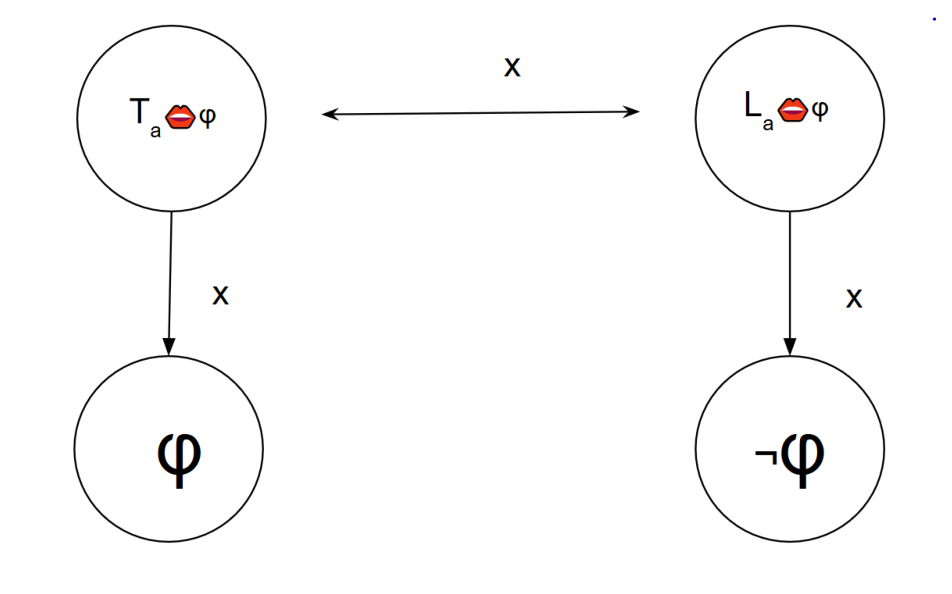
\includegraphics[width=0.5\textwidth]{slide10.eps}
  \caption{Initial space}
\end{figure}\\
\begin{figure}[h!]
  \centering
  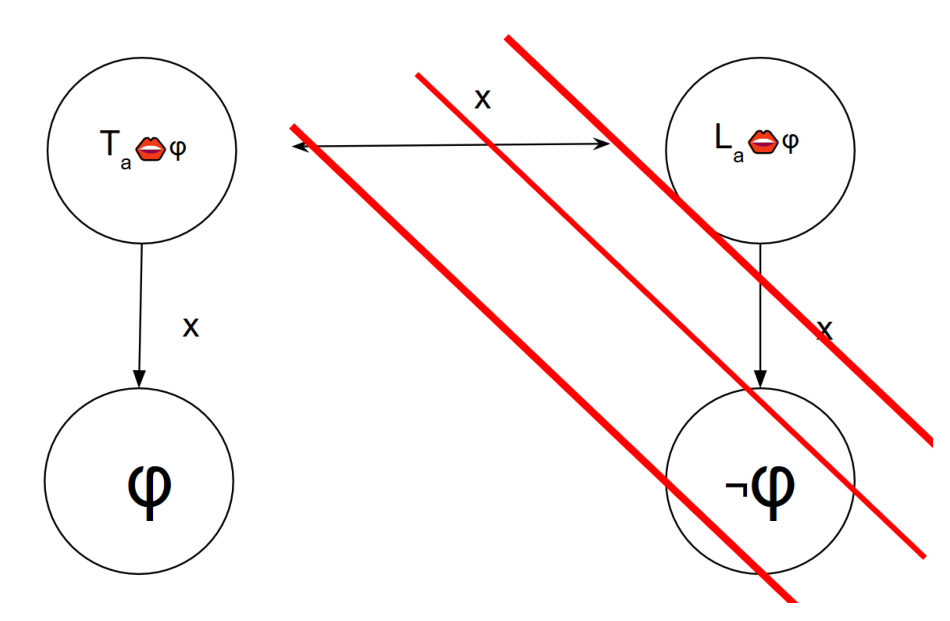
\includegraphics[width=0.5\textwidth]{slide11.eps}
  \caption{After updating with $\psi$}
\end{figure}

\section{Sincere and Insincere Men}
So far this game as appeared straightforward, as in each instance there only exists one possible relationship between the agent's statement and the true state of $\psi$ in the world.\\
Now instead of assuming that you must know $\psi$ in order to be a truth teller, consider instead if all that is required to be a truth teller is to believe $\psi$, as per types 3,4, and 5, with liars being defined equivalently.\\
Unlike omniscient liars and truth-tellers, you cannot identify if someone is sincere or insincere based purely off whether their statement is true in reality.\\
\\
Omniscient Truth-teller:
$$((T_a \text{\textmusicalnote} \psi \to K_a \psi)\to \psi)$$
Sincere Men:
$$((T_a \text{\textmusicalnote} \psi \to B_a \psi)\nrightarrow \psi)$$ \\
Simply put, it is possible for people to have incorrect beliefs.

\subsection{Identification of Sincerity}
If we now use the same framework for our game as we have had previously then we are able to identify if an agent is sincere or insincere;\\
Once the agent $a$ makes their claim 
$$a\text{\textmusicalnote} \psi$$
Then if you know $\psi$, all you need to do is update $a$ to $\psi$.\\
If $a$ knows that all updates are true updates $K_a<!\psi >$
\begin{align*}
&K_a \psi\\
&K_a \psi \to B_a \psi\\
&B_a \psi
\end{align*}
Knowing they now have a belief in $\psi$, if you ask them to repeat their statement they will have to respond in specific ways.\\
A sincere man will always state $a \text{\textmusicalnote} \psi$ as they now believe $\psi$\\
An insincere man will always state $a \text{\textmusicalnote} \neg \psi$ as they now believe $\psi$ with $\tau = \infty$ and as such unless they have a threshold of $0$, they will $\neg B_a \neg \psi$

\section{A 4-Player Game}
%NEED WORK ON FORREST SECTION - SEE QUESTION MARKS (?)
Finally, we look at a game in which the agent can exist in four possible states. The agent can be either:
\begin{itemize}
\item Alan Truering (omniscient truth-teller)
\item Ada Love-Lies (omniscient liar)
\item Sincere man
\item Insincere man
\end{itemize}
If the agent announces $\psi$ you are unable initially to distinguish which state they are in, as per the following model:
%uncomment below and delete this line when image available
%\begin{figure}[h!]
%  \centering
%  \includegraphics[width=0.5\textwidth]{insert_image_here.eps}
%  \caption{$a \text{\textmusicalnote} \psi$}
%\end{figure}
However, if you come to know $\psi$ to be true then you can eliminate Ada Love-Lies from the possible states of $a$ due to her defining proposition: 
$$(K_L \text{\textmusicalnote} \psi \to \neg \psi)$$
Based on the following derivation:
\begin{align*}
&(K_L \text{\textmusicalnote} \psi \wedge \psi )\\
&(K_L \text{\textmusicalnote} \psi )\\
&\psi \\
&(K_L \text{\textmusicalnote} \psi \to \neg \psi )\\
&\neg \psi \\
&\times
\end{align*}
The same format can be used to eliminate Allan Truering if you know $\neg \psi$.\\
Now with the knowledge of $\psi$, you must discern between Alan Truering and the sincere and insincere men.\\
To do this, you must make an announcement. However, unlike the case in which you are restricted to sincere and insincere men you mus not announce $\psi$ - if you do then $\psi$ becomes public knowledge, thereby allowing the sincere man to hold knowledge of $\psi$, making them indistinguishable from Alan Truering.\\
Instead, announce a simple conjunction:
$$(\psi \to K\psi)$$ 
Each agent will evaluate this statement with relation to their own type.\\
For both sincere and insincere men who are simply ???????????
Thus if the agent is sincere they will believe the statement fale and announce $\neg \psi$ as such. $(B_T \text{\textmusicalnote} \neg (K \psi \to \K \psi))$\\
An insincere man will also believe $\neg \psi$to be false???????????
??????
%uncomment below and delete this line when image available
%\begin{figure}[h!]
%  \centering
%  \includegraphics[width=0.5\textwidth]{insert_image_here.eps}
%  \caption{$a \text{\textmusicalnote} \psi$}
%\end{figure}
%NEED WORK ON FORREST SECTION - SEE QUESTION MARKS (?)

\chapter{Gettier Types}
\begin{table}[h]
\begin{tabular}{lp{6cm}p{8cm}}
\hline
   & Description                                                 & Logic                                                                                                           \\ \hline
11 & Gettier Truth-tellers announce truth, for the wrong reasons & (\true$\psi \to ((\neg \chi \wedge \psi ) \wedge B_\tau (\chi \to \psi ) \wedge B_\tau \chi)$)       \\
12 & Gettier Liars announce falsity, for the wrong reasons       & (\false$\neg \psi \to ((\neg \chi \wedge \psi ) \wedge B_\tau (\chi \to \psi ) \wedge B_\tau \chi)$) \\ \hline
\end{tabular}
\end{table}
Based on Van Bentham's notion of a Gettier Truth-teller\autocite{BenthemJohanvan2010Mlfo}, consider a Gettier Truth-teller defined as such; Gettier Truth-tellers announce truth, sincerely, but based on false evidence. They announce $\psi$, which is true in reality, based on some evidence $\chi$, which is false in reality. They make this based on a modus ponens implication of $(\chi \to \psi)$, the only falsity being their belief in $\chi$, which is false.\\
Gettier Liars exist in a similar manner, the primary difference being that they seek to deceive, negating the truth, which they succeed in, but based on evidence that is false.

\section{Gettier Interactions}
From their announcement of $\psi$ as well as your knowledge that they believe $\chi$ falsely, then due to the nature of implication, $(\chi \to \psi)$ holds regardless of the truth value of $\chi$, due to $\psi$ being true. Therefore you can't immediately conclude that they are a Gettier Truth-teller - they may be entirely generic.\\
In order to ascertain them as Gettier, truthfully announce that their (false, but not necessarily known to you) antecedent $\chi$ leads to the negation of a different (true, but not known to them as true) consequent $\rho$,  giving the common knowledge $(\chi \to \neg \rho)$, and they should then be able to make the announcement of their belief in the negation of the (true) consequent $\rho$, i.e. $\neg \rho$, which you know to be a falsehood. This can be modelled as:\\
\begin{figure}[h]
  \centering
  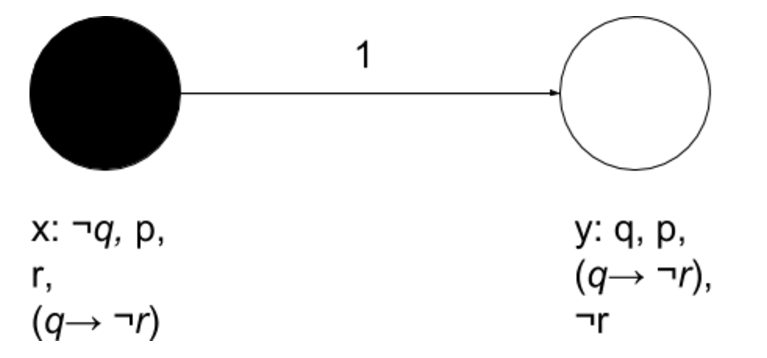
\includegraphics[width=0.5\textwidth]{gettiermodelbase.eps}
  \caption{Plausibility model}
\end{figure}\\
Gettier Liars Interaction is symmetrical to Gettier Truth-tellers - this is not a unique property  of Gettier announcers, however it is worth noting that symmetry isn't common to all types, such as 3,4,5

\subsection{State Plausibility Models}

\begin{figure}[h]
  \centering
  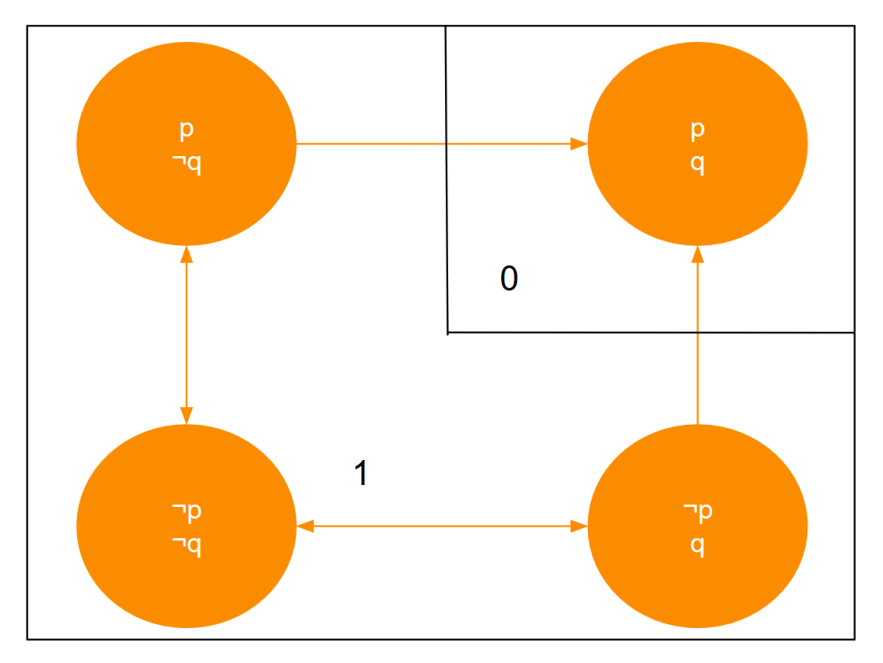
\includegraphics[width=0.5\textwidth]{slide19.eps}
  \caption{Before $(\chi \to \neg \rho)$ announcement, with the derived Spohn rank of states}
\end{figure}

\begin{figure}[h]
  \centering
  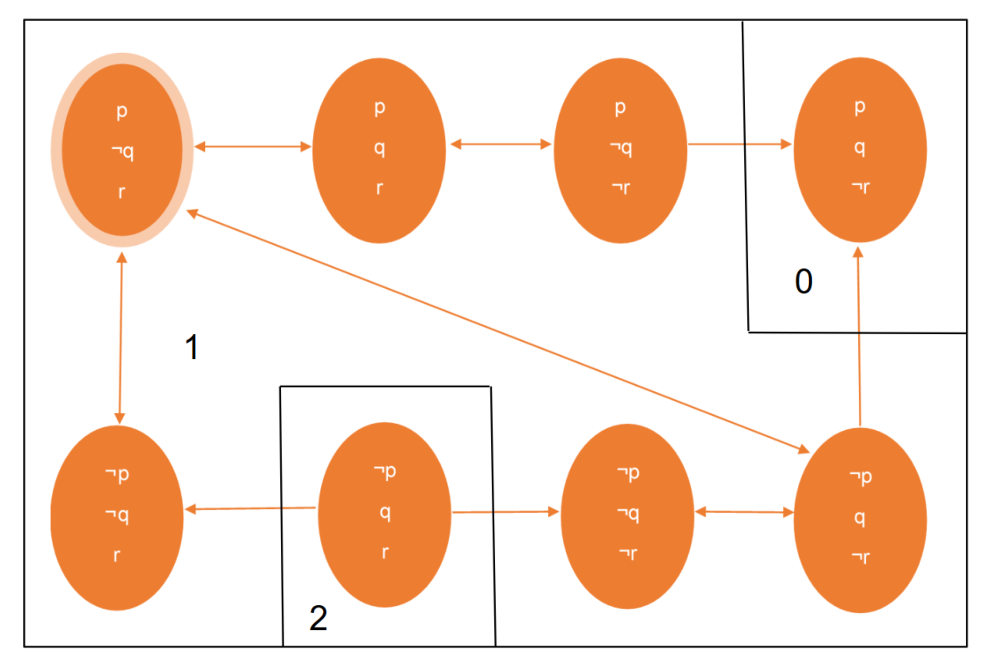
\includegraphics[width=0.5\textwidth]{slide21.eps}
  \caption{After $(\chi \to \neg \rho)$ announcement, with the derived Spohn rank of states}
\end{figure}

\chapter{Non-Gettier Types}
What if you aren't a Gettier Truth-teller? Negating the necessary conditions of Gettier Truth-tellers gives rise to 3 other possible cases when the state of the actual world remains the same. These cases give insight on what other kinds of truth tellers or liars may exist and what might differentiate them.

\section{The Beliefless Truth-teller}
$$((\neg \chi \wedge \psi) \wedge \neg B(\chi \to \psi) \wedge \neg B \chi)$$
In this case, the speaker has no belief in any of the Gettier conditions. The speaker may very well have other types of belief or knowledge that contribute to the announcement of $\psi$, but these are further sub-cases to be examined. If there is no other belief or knowledge that pertains to $\psi$, a speaker satisfying these conditions announces $\psi$ with no rationale or justification. The announcement happens to be true in this world, but that is pure happenstance (when discarding other possible beliefs or knowledge).\\
This case does allow for sub-cases in which the speaker does in fact have a justified true belief in $\psi$ however, as it allows for sub-cases such as:
$$((\neg \chi \wedge \psi) \wedge \neg B(\chi \to \psi) \wedge B \neg \chi)$$

\subsection{State Plausibility Models}
\quad
\newline
\begin{figure}[h!]
  \centering
  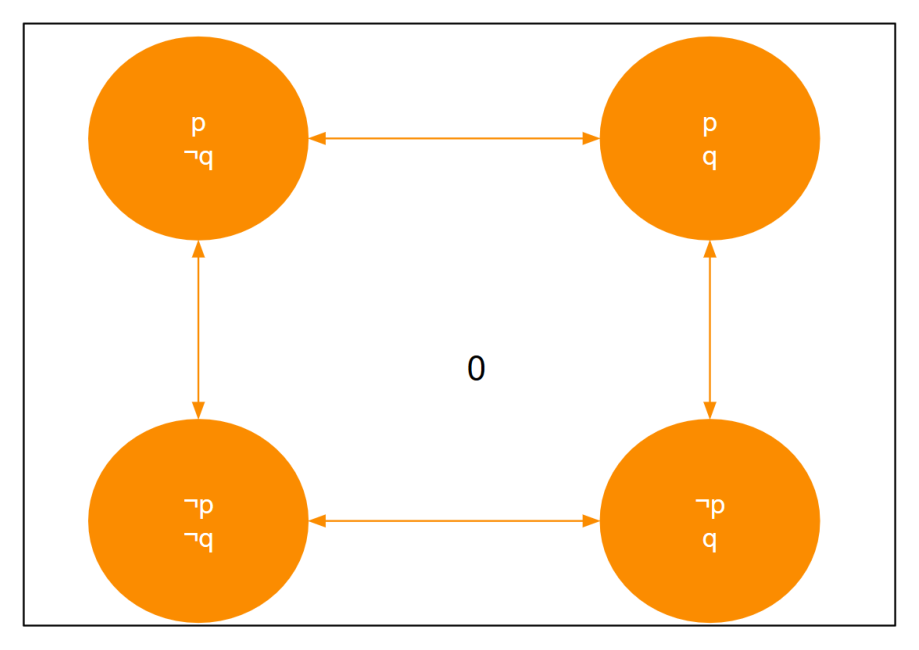
\includegraphics[width=0.5\textwidth]{slide25.eps}
  \caption{Before $(\chi \to \neg \rho)$ announcement, with the derived Spohn rank of states}
\end{figure}
\begin{figure}[h!]
  \centering
  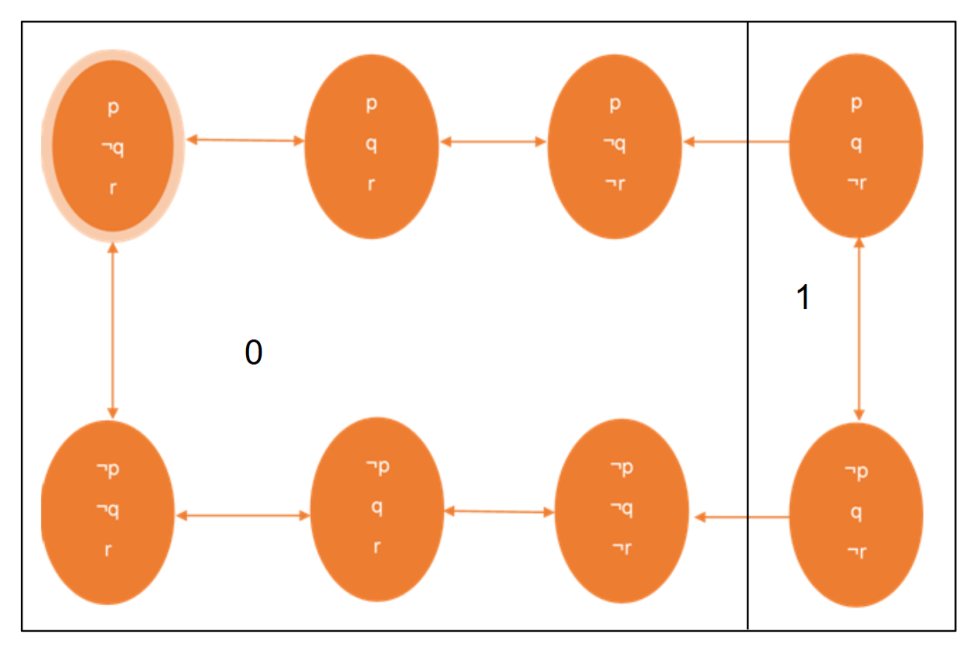
\includegraphics[width=0.5\textwidth]{slide27.eps}
  \caption{After $(\chi \to \neg \rho)$ announcement, with the derived Spohn rank of states}
\end{figure}
\quad
\newline

\section{The Uninformed Accidental Truth-teller}
$$((\neg \chi \wedge \psi) \wedge \neg B(\chi \to \psi) \wedge B \chi)$$
In this case, one has an untrue belief about the world ($B\chi$ when $\neg \chi$), but also doesn't have a belief in the implication $(\chi \to \psi)$ that Gettier Truth Tellers have (a belief which holds true in reality in this state of the world). If one announces $\psi$ with these conditions, they are announcing a true thing but have very little rationale in doing so without considering additional beliefs. They are indifferent on $\psi$ if no other beliefs are held, and therefore announcing $\psi$ seems to be announcing something insincerely. One possible sub-case:
\begin{align*}
&((\neg \chi \wedge \psi) \wedge \neg B(\chi \to \psi) \wedge B \chi \wedge B \neg (\chi \to \psi ))\\
\leftrightarrow &((\neg \chi \wedge \psi) \wedge \neg B(\chi \to \psi) \wedge B \chi \wedge B (\chi \wedge \neg \psi ))\\
\leftrightarrow &((\neg \chi \wedge \psi) \wedge \neg B(\chi \to \psi) \wedge B \chi \wedge B \neg \psi)
\end{align*}
This sub-case is one in which the speaker announcing $\psi$ announces something true about the world, but does so by saying something she believes to be untrue - implying an intent to deceive and a type of lie, but announcing a true statement due to her incorrect beliefs. 

\subsection{State Plausibility Models}
\quad
\newline
\begin{figure}[h!]
  \centering
  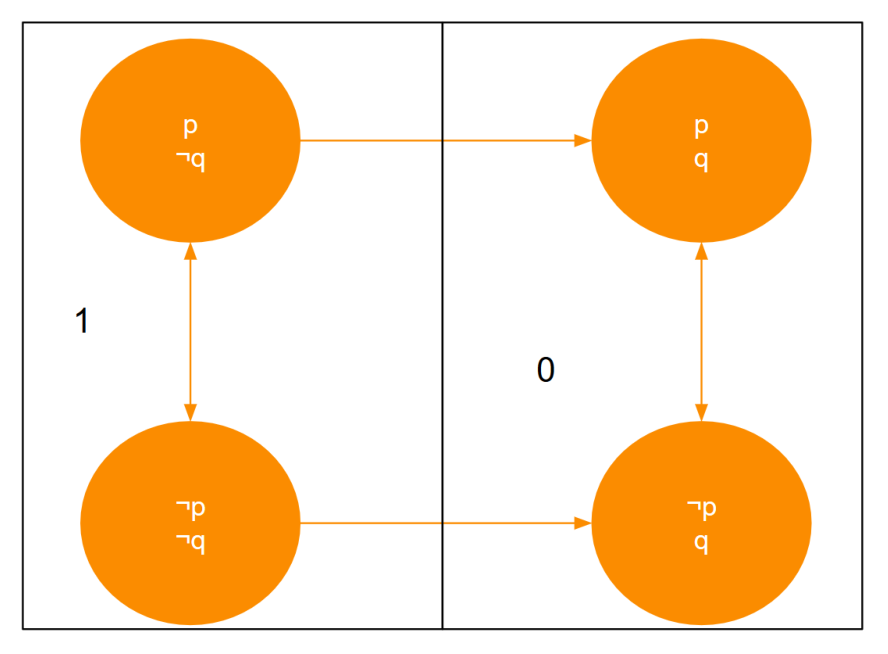
\includegraphics[width=0.5\textwidth]{slide30.eps}
  \caption{Before $(\chi \to \neg \rho)$ announcement, with the derived Spohn rank of states}
\end{figure}
\begin{figure}[h!]
  \centering
  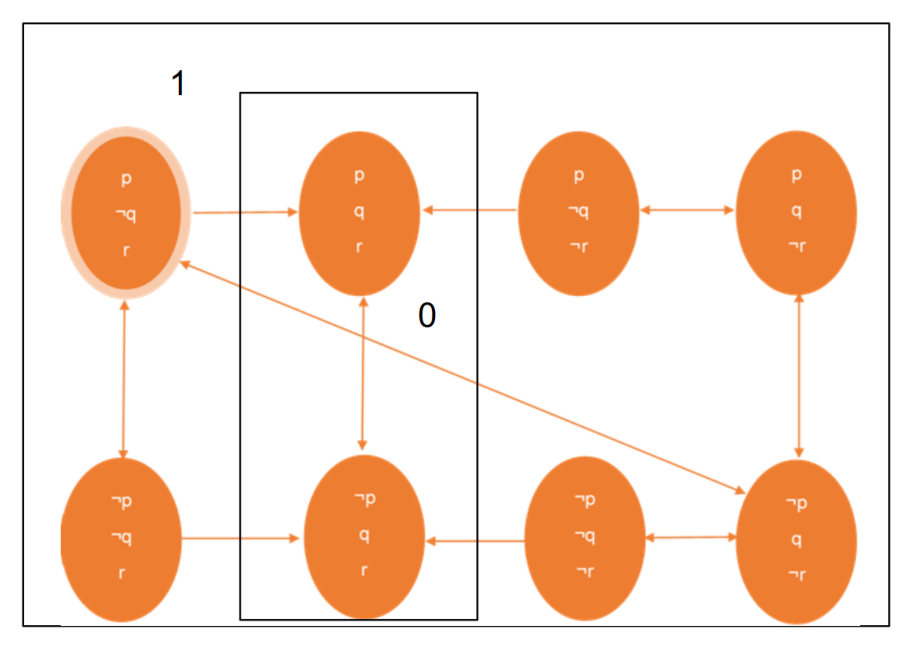
\includegraphics[width=0.5\textwidth]{slide32.eps}
  \caption{After $(\chi \to \neg \rho)$ announcement, with the derived Spohn rank of states}
\end{figure}
\quad
\newline

\section{The Accurate Believer}
$$(\neg \chi \wedge \psi) \wedge B(\chi \to \psi) \wedge \neg B \chi)$$
In this case, announcing $\psi$ is again saying something true, but based on very little evidence without considering other beliefs the speaker may hold. They don’t believe $\chi$, but they do believe $(\chi \to \psi)$, and announcing $\psi$ may be with the intent to deceive if they don't believe $\psi$. This case is one in which the speaker has the most accurate set of beliefs. It is the only case in which the speaker both believes the true statement $(\chi \to \psi)$ and does not falsely believe $\chi$. Interestingly, this case is the only one in which Spohn Rank 0 contains only 5 cases rather than 6. This case allows for sub-cases in which the speaker has a justified true belief of $\psi$ or a justified false belief in $\neg \psi$.

$$(\neg \chi \wedge \psi) \wedge B(\chi \to \psi) \wedge \neg B \chi \wedge B(\psi \to \chi))$$
In this case, one cannot be sincere in announcing $\psi$ as it would then result in $B\chi$ but it is given that $\neg B \chi$

\subsection{State Plausibility Models}
\quad
\newline
\begin{figure}[h!]
  \centering
  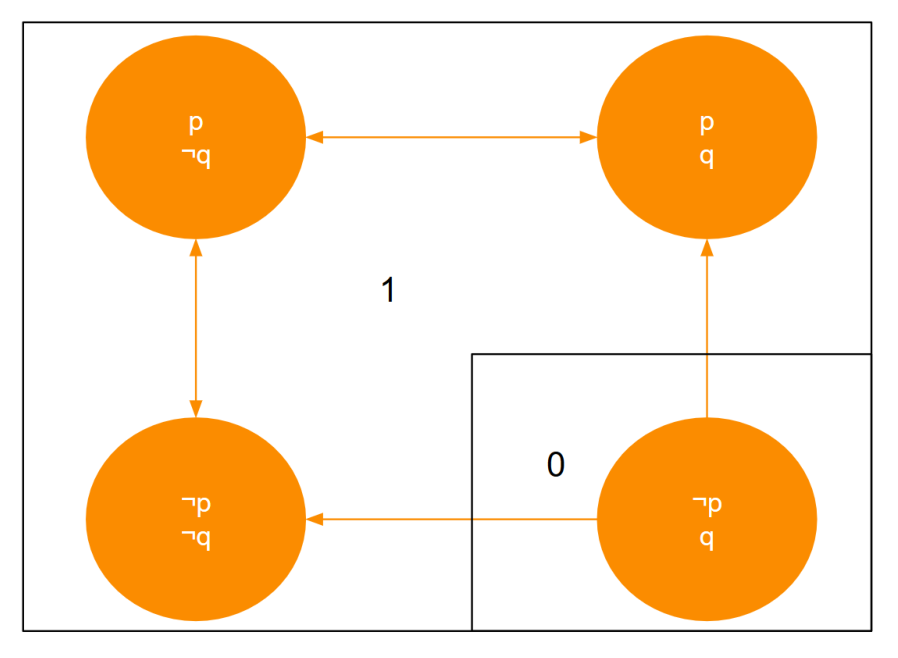
\includegraphics[width=0.5\textwidth]{slide34.eps}
  \caption{Before $(\chi \to \neg \rho)$ announcement, with the derived Spohn rank of states}
\end{figure}
\begin{figure}[h!]
  \centering
  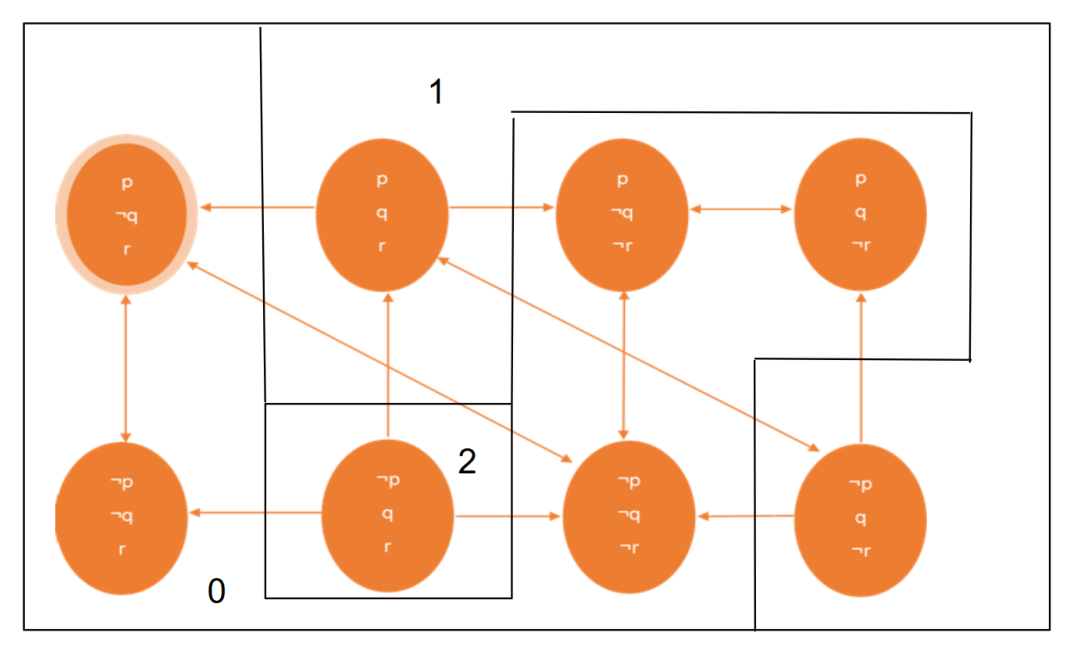
\includegraphics[width=0.5\textwidth]{slide36.eps}
  \caption{After $(\chi \to \neg \rho)$ announcement, with the derived Spohn rank of states}
\end{figure}
\quad
\newline

\chapter{Further Considerations}
Meta:
\begin{itemize}
\item Is there an exhaustive list of liars and truth-tellers?
\item Is it even possible to arrive at one at all?
\end{itemize}
Basic Types:
\begin{itemize}
\item Interactions between omniscient and insincere men
\item How different thresholds affect what can be claimed by sincere and insincere men ($\tau \leq \frac{1}{2}$ and $\tau > \frac{1}{2}$)
\end{itemize}
Building on Gettier and non-Gettier Types:
\begin{itemize}
\item What sub-cases arise from the non-Gettier cases?\item What facets of interaction with these different sub-case agents will differ?
\item Is this non-Gettier approach a useful approach or is too much redundancy embedded in it?
\end{itemize}

\printbibliography
\end{document}
